% !TEX root = ../FundationsDataScience.tex

\chapter{Fourier Transforms}
\label{sec-fourier}

The main references for this chapter is \cite{mallat2008wavelet}.
%
The Fourier transforms offers a perfect blend of analysis (solution of PDEs, approximation of functions), algebra (characters of groups, representation theory) and computer science (the FFT). This chapter offers a glimpse of all these different facets. 

\newcommand{\piN}{\frac{2\imath\pi}{N}}

%%%%%%%%%%%%%%%%%%%%%%%%%%%%%%%%%%%%%%%%%%%%%%%%
%%%%%%%%%%%%%%%%%%%%%%%%%%%%%%%%%%%%%%%%%%%%%%%%
%%%%%%%%%%%%%%%%%%%%%%%%%%%%%%%%%%%%%%%%%%%%%%%%
\section{Hilbert spaces and Fourier Transforms}

%%%%%%%%%%%%%%%%%%%%%%%%%%%%%%%%%%%%%%%%%%%%%%%%
\subsection{Hilbertian bases.}

An Hilbert space $(\Hh,\dotp{\cdot}{\cdot})$ is complete. If it is separable, it can be equipped with an Hilbertian orthogonal basis $(\phi_n)_{n \in \NN}$, which means that one can expand any $f \in \Hh$ as
\eq{
	f = \sum_{n} \dotp{f}{\phi_n} \phi_n 
}
where the convergence is in the sense of $\norm{f}^2 \eqdef \dotp{f}{f}$, i.e. $\norm{ f - \sum_{n=0}^N \dotp{f}{\phi_n} \phi_n } \rightarrow 0$ as $N \rightarrow +\infty$. One also have the conservation of energy 
\eq{
	\norm{f}^2 = \sum_n \dotp{f}{\phi_n}^2.
}

A way to construct such an ortho-basis is using Gram-Schmidt orthogonalization procedure. On $L^2([0,1])$ equipped with the usual inner product, orthogonalization of monomials defines the Legendre polynomials. On $L^2(\RR)$ equipped with a Gaussian measure, this leads to functions of the form $P_n(x) e^{-x^2}$ where $P_n$ are Laguerre polynomials. Intuitively, orthogonality forces $\phi_n$ to have $n$ ``oscillations'', e.g. orthogonal polynomials have exactly $n$ zeros. 

Figure \ref{fig-fourier-wav}, left, shows examples of the real part of Fourier atoms.

\myfigure{
	\image{orthobases}{.4}{atoms-fourier}
	\image{orthobases}{.5}{atoms-wavelets}
}{%
	Left: 1D Fourier (real part), right: wavelet bases. %	
}{fig-fourier-wav}

%%%%%%%%%%%%%%%%%%%%%%%%%%%%%%%%%%%%%%%%%%%%%%%%
\subsection{Fourier basis on $\RR/2\pi\ZZ$.}

On $L^2(\TT)$ where $\TT=\RR/2\pi\ZZ$, equipped with $\dotp{f}{g} \eqdef \frac{1}{2\pi}\int_\TT f(x) \bar g(x) \d x$, one can use the Fourier basis 
\eql{\label{eq-fourier-basis-1d}
	\phi_n(x) \eqdef e^{\imath n x}
	\qforq
	n \in \ZZ. 
}
One thus has
\eql{\label{eq-defn-fourier-coeffs}
	f = \sum_{n} \hat f_n e^{\imath n \cdot}
	\qwhereq
	\hat f_n \eqdef \frac{1}{2\pi}\int_0^{2\pi} f(x) e^{-\imath n x} \d x, 
}
in $L^2(\TT)$ sense. Pointwise convergence is delicate, see Section~\ref{subsec-sampling}.

We recall that for $f \in L^1(\RR)$, its Fourier transform is defined as
\eq{
	\foralls \om \in \RR, \quad
	\hat f(\om) \eqdef \int_\RR f(x) e^{-\imath x \om} \d x.
}
and this is extended to $L^2(\RR)$ by density. 

The connexion between the Fourier transform on $\RR$ and the Fourier coefficients on $\TT$ is given by the following diagram 
\eq{
	\begin{array}{rcccl}
						& f(x)  &  \overset{\Ff}{\longrightarrow} &  \hat f(\om) &\\
		\text{sampling}& \downarrow & & \downarrow &\text{periodization} \\
						& (f(n))_n  &  \overset{\text{Fourier serie}}{\longrightarrow} &  \sum_n f(n) e^{-\imath \om n} &\\
	\end{array}.
}
Its commutativity sates
\eql{\label{eq-poisson-bis}
	\sum_n f(n) e^{-\imath \om n} = \sum_n \hat f(\om-2\pi n)
}
and this is in fact the celebrated Poisson formula (Proposition~\ref{prop-poisson}). 



\myfigure{
\image{fourier}{.8}{fourier-transforms}
}{%
	The four different settings for Fourier analysis, and the sampling-periodization relationship.%	
}{fig-fourier-transforms}



%%%%%%%%%%%%%%%%%%%%%%%%%%%%%%%%%%%%%%%%%%%%%%%%
%%%%%%%%%%%%%%%%%%%%%%%%%%%%%%%%%%%%%%%%%%%%%%%%
%%%%%%%%%%%%%%%%%%%%%%%%%%%%%%%%%%%%%%%%%%%%%%%%
\section{Convolution on $\RR$ and $\TT$}

%%%%%%%%%%%%%%%%%%%%%%%%%%%%%%%%%%%%%%%%%%%%%%%%
\subsection{Convolution}

\wrapf{2-fourier/convolution}{Convolution on $\RR$.}
On $\XX=\RR$ or $\TT$, one defines 
\eql{\label{eq-convol-1d}
	f \star g(x) = \int_\XX f(t) g(x-t) \d t. 
}
Young's inequality shows that this quantity is well defined if $(f,g) \in L^p(\XX) \times L^q(\XX)$
\eql{\label{eq-young-convol}
	\frac{1}{p}+\frac{1}{q}=1+\frac{1}{r} \qarrq
	f \star g \in L^r(\XX) \qandq 
	\norm{f\star g}_{L^r(\XX)} \leq \norm{f}_{L^p(\XX)}\norm{g}_{L^q(\XX)}.
}
This shows that if $f \in L^1(\XX)$, then one has the map $g \in L^p(\XX) \mapsto f \star g \in L^p(\XX)$ is a continuous map on $L^p(\XX)$. Furthermore, when $r=\infty$, $f \star g \in \Cc^0(\XX)$ is a continuous function (which shows some regularizing effect).
%
Note that for $\XX=\TT$, $p<q \qarrq L^q(\TT) \subset L^p(\TT)$, so that $L^\infty(\XX)$ is the smallest space. 


\myfigure{
\image{fourier}{.6}{filtering-principle}
}{%
	Signal filtering with a box filter (running average). %	
}{fig-filter-box}

Convolution is mostly used in order to regularize functions. For instance, if $f \in L^1(\XX)$ and $g \in \Cc^1(\XX)$ is bounded, then $f \star g$ is differentiable and $(f \star g)'=f \star g'$. This is used to produce smooth approximate identity $(\rho_\epsilon = \frac{1}{\epsilon}\rho(\cdot/\epsilon))_\epsilon$ with convergence $f \star \rho_\epsilon \rightarrow f$ in $L^p(\XX)$ for $1 \leq p < +\infty$ of smooth approximations (and convergence in $L^\infty(\XX)$ if $f$ is uniformly continuous). 
%
This is also used for denoising applications in signal and image processing.


\myfigure{
\image{fourier}{.6}{filtering-1d-1}\\
\image{fourier}{.6}{filtering-1d-2}\\
\image{fourier}{.6}{filtering-1d-3}
}{%
	Filtering an irregular signal with a Gaussian filter of increasing filter size $\si$. %	
}{fig-filtering-1d}

%%% FIG %%%
\wrapf{2-fourier/convolution-fourier}{Commutative diagram of convolution-Fourier.}
%%%
For $(f,g) \in L^1(\XX)^2$ (so on $\XX=\TT$, also in any $L^p(\XX)$), one has
\eql{\label{eq-convol-fourier}
	\Ff(f \star g) = \hat f \odot \hat g
} 
which means that $\Ff$ is a morphism of algebra. For instance if $\XX=\RR$, its range is included in the algebra of continuous functions with vanishing limits in $\pm\infty$.

%%%%%%%%%%%%%%%%%%%%%%%%%%%%%%%%%%%%%%%%%%%%%%%%
\subsection{Translation Invariant Operators}

\wrapf{2-fourier/translation-inv}{Commutative diagram for translation invariance.}
Translation invariant operators (which commutes with translation) are fundamental because in most situations, input (signal, image, etc) should be processed without spatial preference.
%
The following propositions shows that any translation invariant\footnote{One should rather actually say ``translation equivariant''.} (i.e. which commutes with translations) operator is actually a ``convolution'' against a distribution with bounded Fourier transform. 
%
The proof and conclusion (regularity of the convolution kernel) vary depending on the topology on the input and output spaces.
%
We first study the case of convolution mapping to continuous functions.

\begin{prop}
	We define $T_\tau f = f(\cdot-\tau)$.
	%
 	A bounded linear operator $H : (L^2(\XX),\norm{\cdot}_2) \rightarrow (C^0(\XX),\norm{\cdot}_\infty)$ is such that for all $\tau$, $H \circ T_\tau = T_\tau \circ H$ if and only if 
	\eq{
		\foralls f \in L^2(\TT), \quad H(f) = f \star g
	}
	with $g \in L^2(\XX)$.
\end{prop}
\begin{proof}
	Thanks to~\eqref{eq-young-convol} (and the remark in the case $r=\infty$), $T : f \mapsto f \star g$ with $g \in L^2(\XX)$ is indeed a continuous operator from $L^2(\XX)$ to $C^0(\XX)$.  Furthermore
	\eq{
		(H \circ T_\tau)(f) = \int_\XX f( (\cdot-\tau)-y) g(y) \d \tau = (f \star g)(\cdot-\tau) = T_\tau (Hf), 
	}
	so that such an $H$ is translation-invariant. 
	
	
	Conversely, we define $\ell : f \mapsto H(f)(0) \in \RR$, which is legit since $H(f) \in \Cc^0(\XX)$. 
	%
	Since $H$ is continuous, there exists $C$ such that $\norm{Hf}_\infty \leq C \norm{f}_2$, and hence $|\ell(f)| \leq C \norm{f}_2$, so that $f$ is a continuous linear form on the Hilbert space $L^2(\XX)$. Hence, according to Fr�chet-Riesz theorem, there exists $h \in L^2(\XX)$ such that $\ell(f)=\dotp{f}{h}$.
	%
	Hence, $\foralls x \in \XX$, 
	\eq{
		H(f)(x) = T_{-x} (Hf)(0) = H ( T_{-x} f)(0) = \ell( T_{-x} f ) = \dotp{T_{-x} f}{h} =
		\int_\XX f(y+x) h(y) \d y = f \star \bar h(x). 
	}
	where $g \eqdef \bar h=h(-\cdot) \in L^2(\XX)$.
\end{proof}

We now study, on $\TT$, the case of convolution which can output non-continuous functions. In this case, the kernel can be a ``distribution'', so the convolution is defined over the Fourier domain. 

\begin{prop}\label{prop-ti-convol-l2}
 	A bounded linear operator $H : L^2(\TT) \rightarrow L^2(\TT)$ is such that for all $\tau$, $H \circ T_\tau = T_\tau \circ H$ if and only if 
	\eq{
		\foralls f \in L^2(\TT), \quad
		\Ff( H(f) ) = \hat f \odot c 
	}
	where $c \in \ell^\infty(\ZZ)$ (a bounded sequence).
\end{prop}
\begin{proof}
	We denote $\phi_n \eqdef e^{\imath n \cdot}$. 
	One has
	\eq{
		H(\phi_n) = e^{\imath n \tau} H(T_\tau(\phi_n)) = e^{\imath n \tau} T_\tau(H(\phi_n)).
	}
	Thus, for all $n$, 
	\eq{
		\dotp{H(\phi_n)}{\phi_m} 
		= e^{\imath n \tau} \dotp{T_\tau \circ H(\phi_n)}{\phi_m} 
		= e^{\imath n \tau} \dotp{H(\phi_n)}{ T_{-\tau}(\phi_m) }
		=  e^{\imath (n-m) \tau} \dotp{H(\phi_n)}{ \phi_m }
	}
	So for $n \neq m$, $\dotp{H(\phi_n)}{\phi_m} = 0$, and we define $c_n \eqdef \dotp{H(\phi_n)}{\phi_n}$. Since $H$ is continuous, $\norm{Hf}_{L^2(\TT)} \leq C \norm{f}_{L^2(\TT)}$ for some constant $C$, and thus
	by Cauchy-Schwartz 
	\eq{
		|c_n| = |\dotp{H(\phi_n)}{\phi_n}| \leq \norm{H(\phi_n)} \norm{\phi_n} \leq C 
	}	
	because $\norm{\phi_n}=1$, so that $c \in \ell^\infty(\ZZ)$.
	%
	By continuity, recalling that by definition $\hat f_n \eqdef \dotp{f}{\phi_n}$, 
	\eq{
		H(f) = \lim_N H( \sum_{n=-N}^N \hat f_n \phi_n ) = \lim_N \sum_{n=-N}^N \hat f_n H(\phi_n)
		= \lim_N \sum_{n=-N}^N c_n \hat f_n \phi_n = \sum_{n \in \ZZ} c_n \hat f_n \phi_n
	} 
	so that in particular one has the desired result.
\end{proof}

This theorem thus states that translation invariant operators are those which are ``diagonal'' in the Fourier ortho-basis. 

%%%%%%%%%%%%%%%%%%%%%%%%%%%%%%%%%%%%%%%%%%%%%%%%
\subsection{Revisiting Poisson formula using distributions.}

Informally, the Fourier series
\eq{
	\sum_n f(n) e^{-\imath \om n}
} 
can be thought as the Fourier transform $\Ff( \Pi_1 \odot f )$ of the discrete distribution
\eq{
	\Pi_1 \odot f = \sum_n f(n) \de_{n}
	\qwhereq
	\Pi_s = \sum_n \de_{sn}
}
for $s \in \RR$, 
where $\de_a$ is the Dirac mass at location $a \in \RR$, i.e. the distribution such that $\int f \d(\d_a)=f(a)$ for any continuous $f$. Indeed, one can multiply a distribution by a continuous function, and the definition of the Fourier transform of a distribution $\mu$ is a distributions $\Ff(\mu)$ such that that 
\eq{
	\foralls g \in \Ss(\RR), \quad \int_\RR g(x) \d \Ff(\mu) = \int_\RR \Ff^*(g) \d \mu, 
	\qwhereq
	\Ff^*(g) \eqdef \int_\RR g(x) e^{\imath x \cdot} \d x, 
}
where $\Ss(\RR)$ are smooth and rapidly decaying (Schwartz class) functions.

\wrapf{2-fourier/poisson-distrib}{Sine wave being summed in the Poisson formula.}
The Poisson formula~\eqref{eq-poisson-bis} can thus be interpreted as
\eq{
	\Ff(\Pi_1 \odot f) = \sum_n \hat f(\cdot-2\pi n) = \int_\RR \hat f(\cdot-\om) \d\Pi_{2\pi}(\om)  = \hat f \star \Pi_{2\pi}
}
Since $\Ff^{-1} = \frac{1}{2\pi} \Ss \circ \Ff$ where $\Ss(f)=f(-\cdot)$, one has, applying this operator on both sides
\eq{
	\Pi_1 \odot f = \frac{1}{2\pi}�\Ss \circ \Ff(\hat f \star \Pi_{2\pi}) =  \Ss(  \frac{1}{2\pi} \Ff(\hat f) \odot \hat\Pi_{2\pi})
	= \Ss(  \frac{1}{2\pi} \Ff(\hat f) ) \odot \Ss(\hat\Pi_{2\pi}) = \hat \Pi_{2\pi} \odot f.
}
This can be interpreted as the relation
\eq{
	\hat\Pi_{2\pi} = \Pi_{1}
	\qarrq
	\hat\Pi_1 = 2\pi \Pi_{2\pi}.
}

To intuitively understand this relation, one can compute a finite Fourier series
\eq{
	\sum_{n=-N}^N e^{-\imath n \om} = \frac{ \sin( (N+1/2) x) }{\sin(x/2)}
}
which is a smooth function which grows unbounded with $N \rightarrow +\infty$ as $N \rightarrow +\infty$. 

%%%%%%%%%%%%%%%%%%%%%%%%%%%%%%%%%%%%%%%%%%%%%%%%
%%%%%%%%%%%%%%%%%%%%%%%%%%%%%%%%%%%%%%%%%%%%%%%%
%%%%%%%%%%%%%%%%%%%%%%%%%%%%%%%%%%%%%%%%%%%%%%%%
\section{Finite Fourier Transform and Convolution}


%%%%%%%%%%%%%%%%%%%%%%%%%%%%%%%%%%%%%%%%%%%
\subsection{Discrete Ortho-bases}

Discrete signals are finite dimensional vector $f \in \CC^N$ where $N$ is the number of samples and where each $f[n]$ is the value of the signal at a 1D or 2D location. For a 2-D images $f \in \CC^N \simeq \CC^{N_0 \times N_0}$, $N = N_0 \times N_0$, where $N_0$ is the number of pixels along each direction.

Discrete signals and images are processed using a discrete inner product that mimics the continuous $\Ldeux$ inner product
\eq{
	\dotp{f}{g} = \sum_{n=0}^{N-1} f[n] \bar g[n].
}
One thus defines a distance between discretized vectors as
\eq{
	\norm{f-g}^2 = \sum_{n=0}^{N-1} |f[n]-g[n]|^2.
}

Exactly as in the continuous case, a discrete orthogonal basis $\{ \psi_m \}_{0 \leq m < N }$ of $\CC^N$, satisfies
\eql{\label{eq-orthobasis-disc}
	\dotp{\psi_m}{\psi_{m'}} = \de[m-m'].
}
The decomposition of a signal in such an ortho-basis is written
\eq{
	f = \sum_{m=0}^{N-1} \dotp{f}{\psi_m} \psi_m.
}
It satisfies a conservation of energy
\eq{
	\norm{f}^2 = \sum_{n=0}^{N-1} |f[n]|^2 = 
\sum_{m=0}^{N-1} |\dotp{f}{\psi_m}|^2
}

Computing the set of all inner product $\{\dotp{f}{\psi_m}\}_{0 \leq m < N}$ is done in a brute force way in $O(N^2)$ operations.
This is not feasible for large datasets where $N$ is of the order of millions. When designing an ortho-basis, one should keep this limitation in mind and enforce some structure in the basis elements so that the decomposition can be computed with fast algorithm. This is the case for the Fourier and wavelet bases, that enjoy respectively $O(N\log(N))$ and $O(N)$ algorithms.


%%%%%%%%%%%%%%%%%%%%%%%%%%%%%%%%%%%%%%%%%%%%%%%%
\subsection{Discrete Fourier transform}

We denote $f = (f_n)_{n=0}^{N-1}�\in \RR^N$, but we insists that such vector should really be understood as being indexed by $n \in \ZZ/N\ZZ$, which is a finite commutative group for the addition. This corresponds to using periodic boundary conditions. 

The discrete Fourier transform is defined as
\eql{\label{eq-dft}
	\foralls k=0,\ldots,N-1, \quad \hat f_k \eqdef \sum_{n=0}^{N-1} f_n e^{-\piN kn} = \dotp{f}{\phi_k}
	\qwhereq
	\phi_k \eqdef ( e^{\piN kn} )_{n=0}^{N-1} \in \CC^N
}
where the canonical inner product on $\CC^N$ is $\dotp{u}{v}=\sum_{n=1}^N u_n \bar v_n$ for $(u,v) \in (\CC^N)^2$.
%
This definition can intuitively be motivated by sampling the Fourier basis $x \mapsto e^{\imath k x}$ on $\RR/2\pi\ZZ$ at equi-spaced points $( \frac{2\pi}{N}n )_{n=0}^{N-1}$.
%
The following proposition shows that this corresponds to a decomposition in an ortho-basis.

\begin{prop}
	One has
	\eq{
		\dotp{\phi_k}{\phi_\ell} = \choice{
			N \qifq k=\ell, \\
			0 \quad\text{otherwise.}
		}
	}
	In particular, this implies
	\eql{\label{eq-dft-inv}
		\foralls n=0,\ldots,N-1, \quad
		f_n = \frac{1}{N}\sum_k \hat f_k e^{\piN kn}. 
	}
\end{prop}
\begin{proof}
	One has, if $k \neq \ell$
	\eq{
		\dotp{\phi_k}{\phi_\ell} = \sum_n e^{\piN (k-\ell) n} = 
		\frac{ 1 - e^{\piN (k-\ell) N} }{ 1 - e^{\piN (k-\ell)} } = 0
	}
	which is the sum of a geometric serie (equivalently, sum of equi-spaced points on a circle). 
	%
	The inversion formula is simply $f = \sum_k \dotp{f}{\phi_k} \frac{\phi_k}{\norm{\phi_k}^2}$.
\end{proof}


%%%%%%%%%%%%%%%%%%%%%%%%%%%%%%%%%%%%%%%%%%%%%%%%
\subsection{Fast Fourier transform}

Assuming $N=2N'$, one has 
\begin{align*}
	\hat f_{2k} &= \sum_{n=0}^{N'-1} (f_n + f_{n+N/2}) e^{ -\frac{2\imath\pi}{N'} k n } \\
	\hat f_{2k+1} &= \sum_{n=0}^{N'-1} e^{ -\frac{2\imath\pi}{N'} n } (f_n - f_{n+N/2}) e^{ -\frac{2\imath\pi}{N'} k n }.
\end{align*}
For the second line, we used the computation
\eq{
	e^{-\frac{2\imath\pi}{N}(2k+1)(n+N/2)} =
	e^{-\frac{2\imath\pi}{N}(2kn+kN+n+N/2)} = - e^{ -\frac{2\imath\pi}{N'} n } e^{ -\frac{2\imath\pi}{N'} k n }.
}
Denoting $\Ff_N(f)=\hat f$ the discrete Fourier transform on $\RR^N$, and 
introducing the notation $f_e = (f_n + f_{n+N/2})_n \in \RR^{N'}$, $f_o = (f_n - f_{n+N/2})_n \in \RR^{N'}$
and $\al_N = (  e^{ -\frac{2\imath\pi}{N'} n } )_{n} \in \RR^{N'}$, one has the following recursion formula
\eq{
	\Ff_N(f) = \Ii_N( \Ff_{N/2}(f_e), \Ff_{N/2}(f_o \odot \al_N) )
}
where $\Ii_N$ is the ``interleaving'' operator, defined by $\Ii_N(a,b) \eqdef (a_1,b_1,a_2,b_2,\ldots,a_{N'},b_{N'})$.
%
There iterations define the so-called Fast Fourier Transform algorithm, which works here when $N$ is a power of 2. These iterations can be extended to arbitrary number $N$, but a workaround is to simply pad with 0 (or use more complicated extensions) to have vector with size that are power of $2$. 

\begin{figure}
\centering
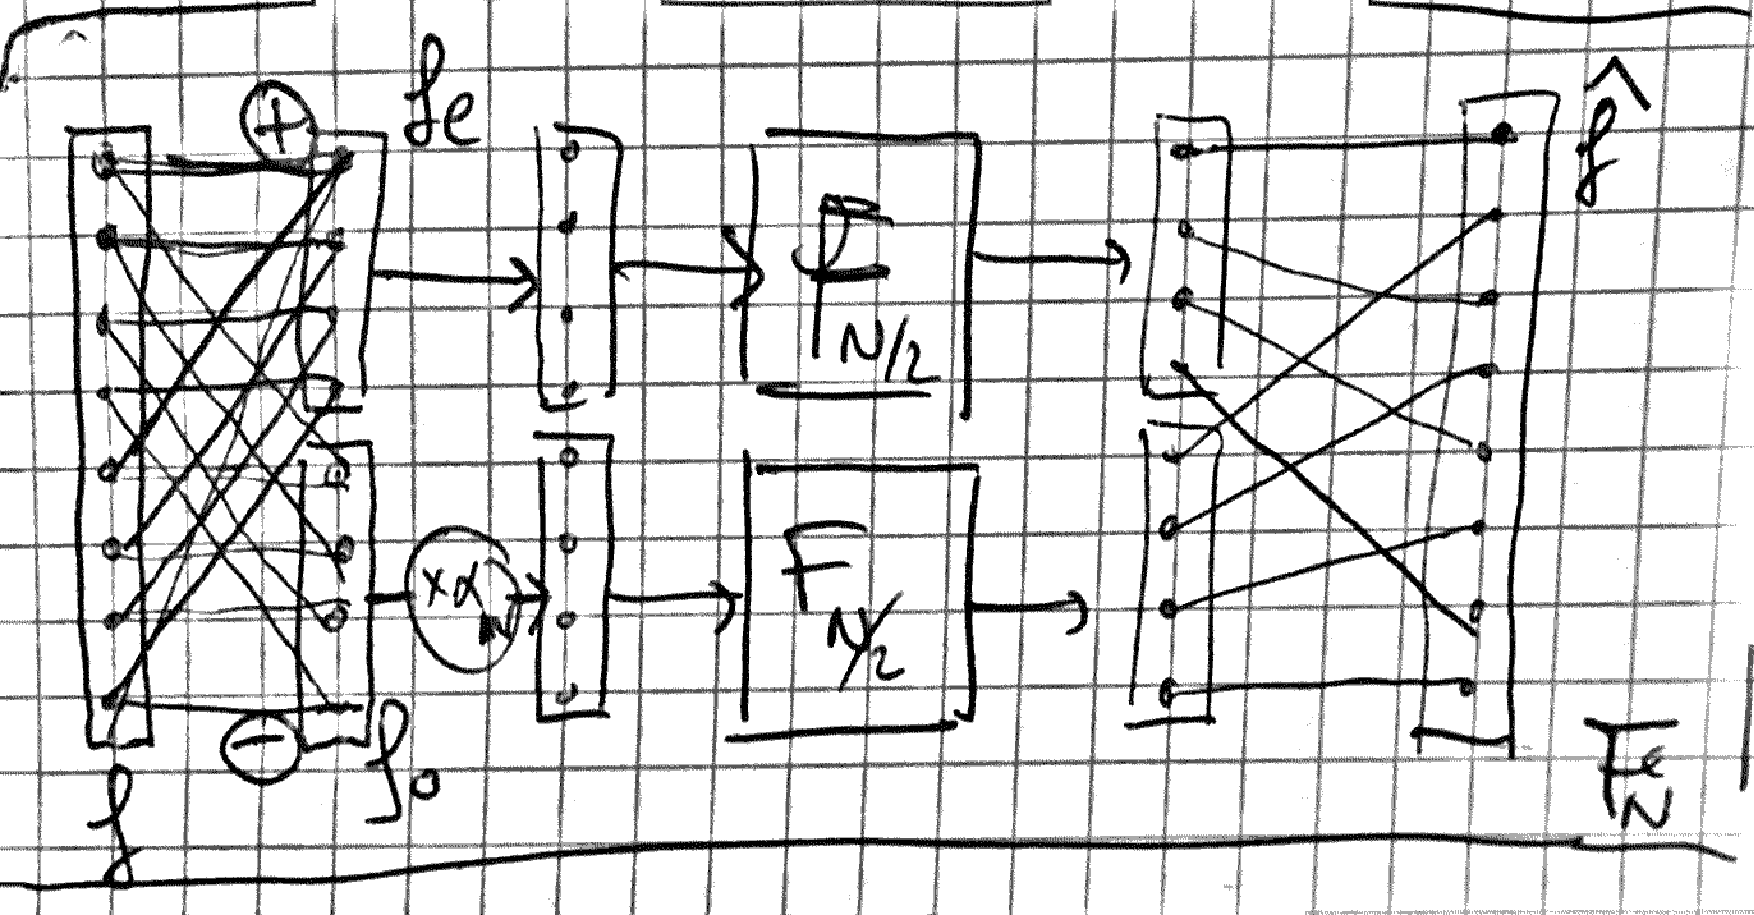
\includegraphics[width=.5\linewidth]{2-fourier/fft}
\caption{\label{fig-fft}
Diagram of one step of the FFT.
}
\end{figure}
 

Denoting $C(N)$ the numerical complexity (number of elementary operations) associated to the computation of $\hat f$, one thus has
\eql{\label{eq-cplx-fft}
	C(N) = 2C(N/2)+NK
}
where $K$ is the complexity of $N$ complex additions and $N/2$ multiplications. Making the change of variable 
\eq{
	\ell \eqdef \log_2(N)
	\qandq 
	T(\ell) \eqdef \frac{C(N)}{N}
}
i.e. $C(N)=2^\ell T(\ell)$, the relation~\eqref{eq-cplx-fft} becomes
\eq{
	2^\ell T(\ell) = 2 \times 2^{\ell-1} T(\ell-1) + 2^\ell K \qarrq
	T(\ell) = T(\ell-1) + K \qarrq
	T(\ell) = T(0) + K \ell
} 
and using the fact that $T(0)=C(1)/1=0$, one obtains
\eq{
	C(N) = K N \log_2(N).
}
This complexity should be contrasted with the complexity $O(N^2)$ of directly computing the $N$ coefficients~\eqref{eq-dft}, each involving a sum of size $N$. 


%%%%%%%%%%%%%%%%%%%%%%%%%%%%%%%%%%%%%%%%%%%%%%%%
\subsection{Finite convolution}

For $(f,g) \in (\RR^{N})^2$, one defines $f\star g \in \RR^N$ as
\eql{\label{eq-finite-convol}
	\foralls n=0,\ldots,N-1, \quad
	(f \star g)_n \eqdef \sum_{k=0}^{N-1} f_k g_{n-k} = \sum_{k+\ell=n} f_k g_\ell 
}
where one should be careful that here $+$ and $-$ should be understood modulo $N$ (vectors should be seen as being defined on the group $\ZZ/N\ZZ$, or equivalently, one uses periodic boundary conditions).
%
This defines an commutative algebra structure $(\RR^N,+,\star)$, with neutral element the ``Dirac'' $\de_0 \eqdef (1,0,\ldots,0)^\top \in \RR^N$. The following proposition shows that $\Ff : f \mapsto \hat f$ is an algebra bijective isometry (up to a scaling by $\sqrt{N}$ of the norm) mapping to $(\RR^N,+,\odot)$ with neutral element $\ones_N=(1,\ldots,1) \in \RR^N$.

\begin{prop}\label{prop-tfd-conv}
	One has $\Ff( f \star g ) = \hat f \odot \hat g$. 
\end{prop}
\begin{proof}
	We denote $T : g \mapsto f \star g$. One has 
	\eq{
		(T \phi_\ell)_n = \sum_k f_k e^{ \piN \ell(n-k) } = e^{ \piN \ell n } \hat f_\ell.
	}
	This shows that $(\phi_\ell)_\ell$ are the $N$ eigenvectors of $T$ with associated eigenvalues $\hat f_\ell$. So $T$ is diagonalizable in this basis. Denoting $F=(  e^{ -\piN k n } )_{k,n}$ the matrix of the Fourier transform, the Fourier inversion formula~\eqref{eq-dft-inv} reads $F^{-1} = \frac{1}{N}F^*$ where $F^*=\bar F^\top$ is the adjoint matrix (trans-conjugate). The diagonalization of $T$ now reads
	\eq{
		T = F^{-1} \diag(\hat f) F =  \qarrq
		\Ff(T g) = \diag(\hat f) F g \qarrq
		\Ff(f \star g) = \diag(\hat f) \hat g.
	} 
\end{proof}

This proposition shows that one can compute in $O(N\log(N))$ operation via the formula
\eq{	
	f \star g = \FF^{-1}( \hat f \odot \hat g ).
}
This is very advantageous with respect to the naive implementation of formula~\eqref{eq-finite-convol}, in the case where $f$ and $g$ have large support. In case where $|\Supp(g)|=P$ is small, then direct implementation is $O(PN)$ which might be advantageous. An example is $g=[1,1,0,\ldots,0,1]/3$, the moving average, where
\eq{
	(f \star g)_n = \frac{f_{n-1}+f_n+f_{n+1}}{3}
}
needs $3N$ operations.

An example of application of the FFT is the multiplication of large polynomial, and thus of large integers (viewing the expansion in a certain basis as a polynomial). Indeed
\eq{
	(\sum_{i=0}^A a_i X_i)( \sum_{j=0}^B b_i X^j ) = 
	\sum_{k=0}^{A+B} ( \sum_{i+j=k} a_i b_j ) X^k
}
One can write $\sum_{i+j=k} a_i b_j = (\bar a \star \bar b)_k$ when one defines $\bar a,\bar b \in \RR^{A+B}$ by zero padding. 


%%%%%%%%%%%%%%%%%%%%%%%%%%%%%%%%%%%%%%%%%%%%%%%%
%%%%%%%%%%%%%%%%%%%%%%%%%%%%%%%%%%%%%%%%%%%%%%%%
%%%%%%%%%%%%%%%%%%%%%%%%%%%%%%%%%%%%%%%%%%%%%%%%
\section{Discretisation Issues}
\label{sec-fourier-discretization}

Beside computing convolutions, another major application of the FFT is to approximate the Fourier transform and its inverse, thus leading to a computationally efficient spectral interpolation method.


%%%%%%%%%%%%%%%%%%%%%%%%%%%%%%%%%%%%%%%%%%%%%%%%
\subsection{Fourier approximation via spatial zero padding.}

It is possible to view the discrete finite Fourier transform~\eqref{eq-dft} as a first order approximation to compute Fourier coefficients, or rather actually samples from the Fourier transform~\eqref{eq-fourier-transform}. Supposing that $f$ is a smooth enough function is supported on $[0,1]$, we consider the discrete Fourier transform of the vector $f^Q \eqdef (f(n/N))_{n=0^{Q-1}} \in \RR^Q$  where $Q \geq N$ induced a padding by $0$ (since $f(n/N)=0$ for $n > N$)
\eq{
	\foralls k \in \range{-\frac{Q}{2},\frac{Q}{2}}, \quad
	\frac{1}{N} \hat f_k^Q = \frac{1}{N} \sum_{n=0}^{N-1} f\pa{\frac{n}{N}} e^{-\frac{2\imath\pi}{Q} n k}
	\approx \int_0^1 f(x) e^{-\frac{2 k\imath\pi}{T} x} \d x = \hat f\pa{\frac{2 k \pi}{T}}
	\qwhereq
	T \eqdef \frac{Q}{N}.
}
The approximation is first order accurate, i.e. $O(1/N)$ for a $C^1$ function $f$. Increasing the amount $Q$ of zero padding is a way to compute larger frequencies. Increasing the discretization precision $N$ is on contrary a way to increase the precision of the Fourier sampling (using smaller step size $2\pi/T$). 

\begin{figure}
\centering
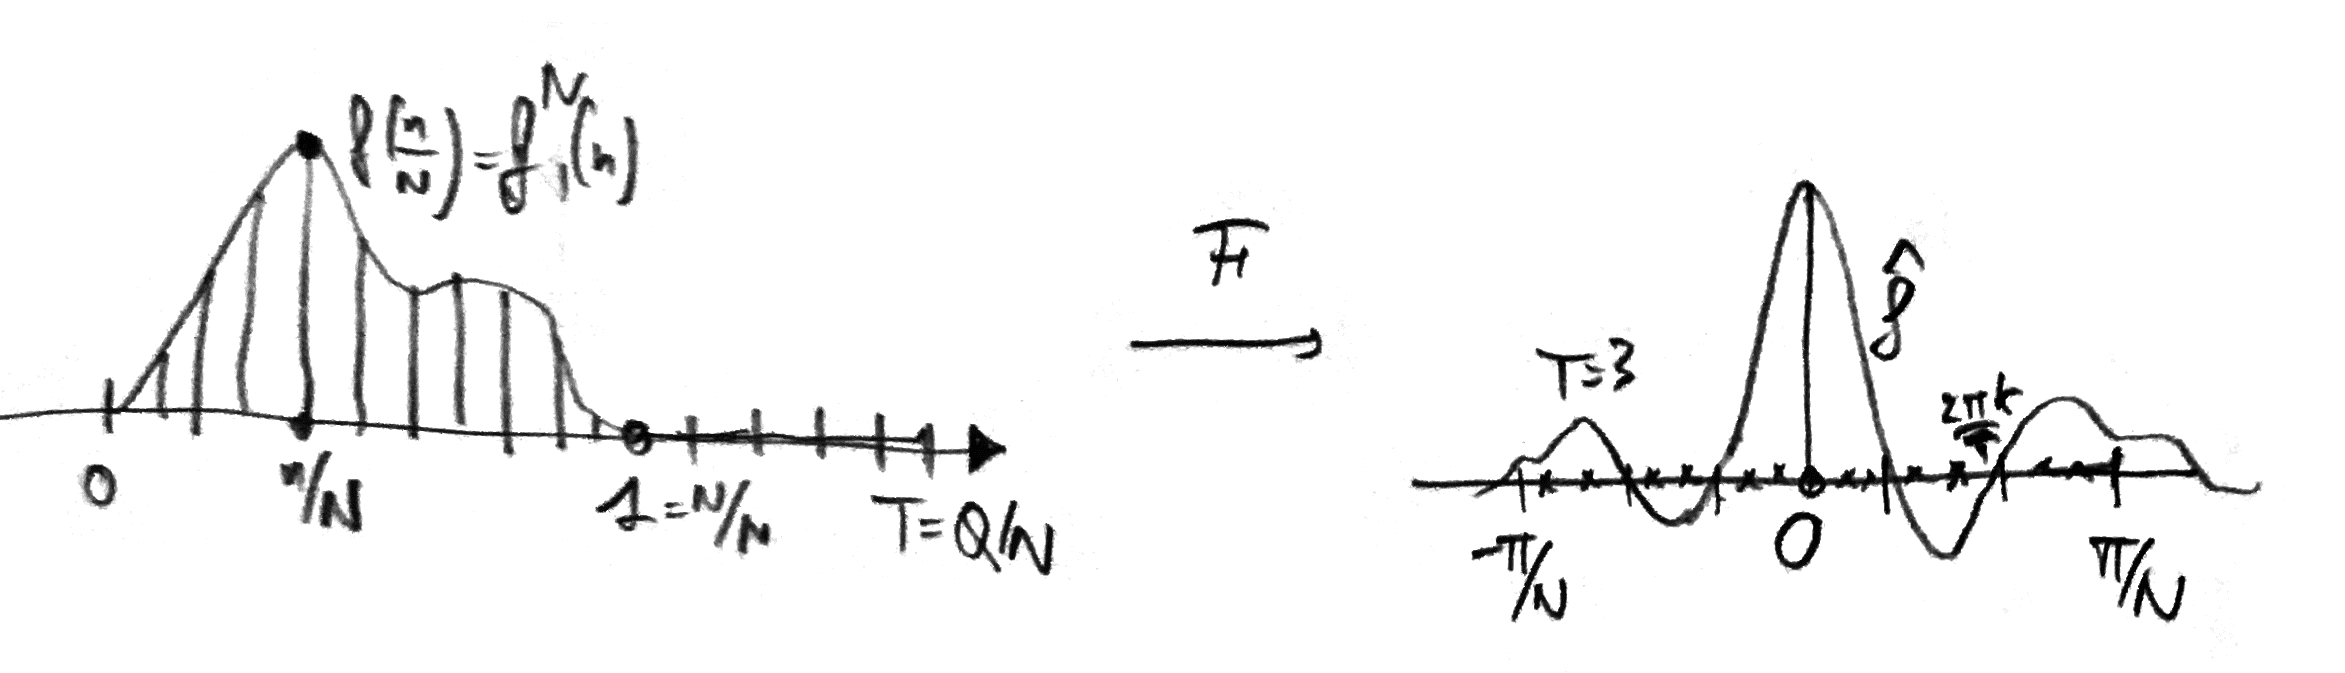
\includegraphics[width=.75\linewidth]{2-fourier/padding-spacial}
\caption{\label{fig-padding-spacial}
Fourier transform approximation by zero-padding in the spatial domain.
}
\end{figure}


%%%%%%%%%%%%%%%%%%%%%%%%%%%%%%%%%%%%%%%%%%%%%%%%
\subsection{Fourier approximation via spatial zero padding.}

If one has at its disposal $N$ uniform discrete samples $f^N=(f^N_n)_{n=0}^{N-1}$, one can compute its discrete Fourier transform $\Ff(f^N) = \hat f^N$ (in $O(N \log(N))$ operations with the FFT), 
\eq{
	\hat f^N_k \eqdef \sum_{n=0}^{N-1} f^N_n e^{-\frac{2\imath\pi}{N} n k}, 
}
and then zero-pad it to obtain a vector of length $Q$.
%
For simplicity, we assume $N=2N'+1$ is odd, and this computation can be also done (but is more involved) with even size.
%
Indexing the frequencies as $-N' \leq k \leq N'$ The padding vector is of the form, 
\eq{
	\tilde f^Q \eqdef (0,\ldots,0,\hat f^N,0,\ldots,0) \in \RR^Q
} 
One can then compute the (with a normalization constant $Q/N$) inverse discrete Fourier transform of size $Q$ (in $O(Q \log(Q))$ operations with the FFT) to obtain
\begin{align*}
	\frac{Q}{N} \Ff^{-1}( \tilde f^Q )_\ell &= 
	\frac{Q}{N} \times \frac{1}{N} \sum_{k=-N'}^{N'} \hat f_k^N e^{ \frac{2\imath\pi}{Q} \ell k } 
	= \frac{1}{N} \sum_{k=-N'}^{N'} \sum_{n=0}^{N-1} f^N_n e^{\frac{2\imath\pi}{N} n k} e^{ \frac{2\imath\pi}{Q} \ell k }  \\
	&= \sum_{n=0}^{N-1} f^N_n \frac{1}{N} \sum_{k=-N'}^{N'} e^{ 2\imath\pi \pa{ -\frac{n}{N} + \frac{\ell}{Q} } k } 
	=  \sum_{n=0}^{N-1} f^N_n 
			\frac{ 
				\sin\left[ \pi N \pa{ \frac{\ell}{Q} - \frac{n}{N} } \right]  
			}{
				N \sin\left[ \pi \pa{ \frac{\ell}{Q} - \frac{n}{N} } \right]
			}  \\
	&= \sum_{n=0}^{N-1} f^N_n \sinc_N\pa{ \frac{\ell}{T} - n }
	\qwhereq
	T \eqdef \frac{Q}{N} \qandq \sinc_N(u) \eqdef \frac{ \sin(\pi u) }{ N \sin(\pi u /N) }.
\end{align*}
Here we use the following summation rule for geometric series for $\rho=e^{\imath \om}$, $a=-b$, $\om = 2\pi \pa{ -\frac{n}{N} + \frac{\ell}{Q} }$, 
\eq{
	\sum_{i=a}^b \rho^i = \frac{ \rho^{a-\frac{1}{2}} - \rho^{b+\frac{1}{2}} }{ \rho^{-\frac{1}{2}} - \rho^{\frac{1}{2}} }
	= \frac{ \sin( (b+\frac{1}{2}) \om ) }{ \sin(\om/2) }.
}
This zero-padding method leads to a discrete version of the Shannon interpolation formula~\eqref{eq-shannong-interp}, which allows to comput the interpolation on a grid of size $Q$ are cost $O(Q\log(Q))$. Increasing $N$ increases the accuracy of the formula, since $\sinc_N \rightarrow \sinc$ as $N \rightarrow +\infty$.

\begin{figure}
\centering
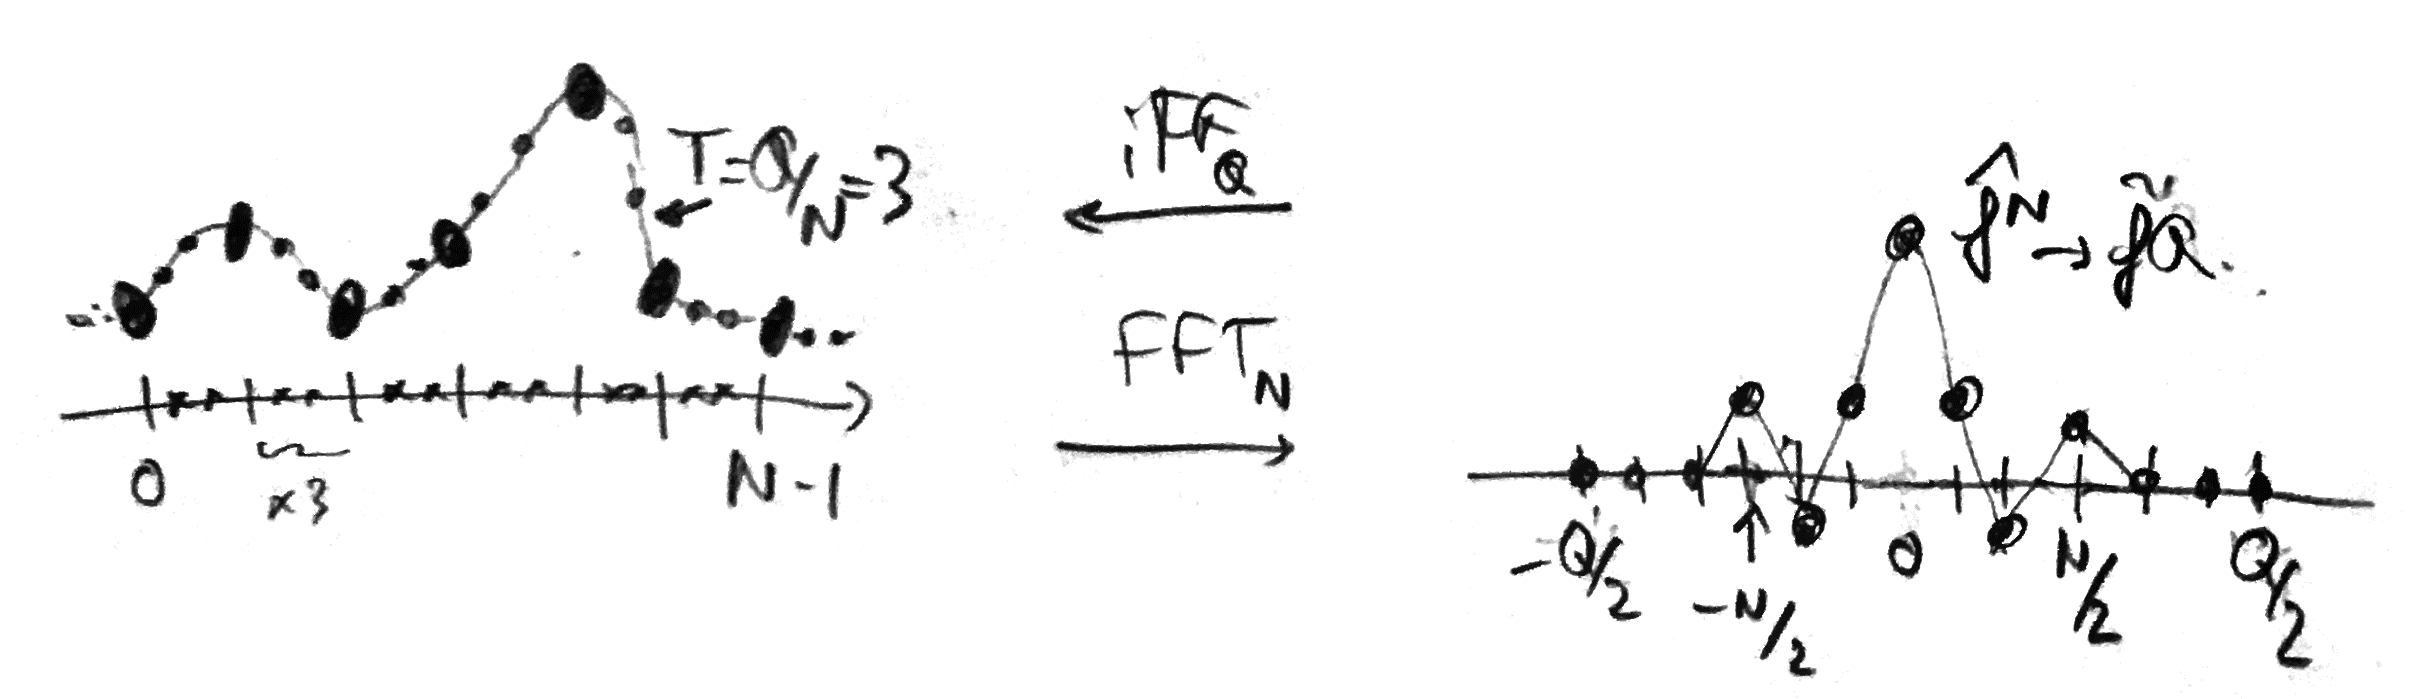
\includegraphics[width=.75\linewidth]{2-fourier/padding-fourier}
\caption{\label{fig-padding-fourier}
Interpolation by zero-padding in the frequency domain.
}
\end{figure}

%%%%%%%%%%%%%%%%%%%%%%%%%%%%%%%%%%%%%%%%%%%%%%%%
%%%%%%%%%%%%%%%%%%%%%%%%%%%%%%%%%%%%%%%%%%%%%%%%
%%%%%%%%%%%%%%%%%%%%%%%%%%%%%%%%%%%%%%%%%%%%%%%%
\section{Fourier in Multiple Dimensions}
\label{sec-fourier-multiple-dim}

The Fourier transform is extended from 1-D to arbitrary finite dimension $d>1$ by tensor product. 


%%%%%%%%%%%%%%%%%%%%%%%%%%%%%%%%%%%%%%%%%%%%%%%%
\subsection{On Continuous Domains}

%%%
\paragraph{On $\RR^d$.}

\wrapf{2-fourier/wave}{2-D sine wave.}
The crux of the power of Fourier transform in arbitrary dimension is that a product of elementary 1-D sine waves is still a sine wave
\eq{
	\prod_{\ell=1}^d e^{ \imath x_\ell \om_\ell } = e^{ \imath \dotp{x}{\om} }
}
moving orthogonally to the wave vector $\om=(\om_\ell)_{\ell=1}^d \in \RR^d$. Here $\dotp{x}{\om} = \sum_\ell x_\ell \om_\ell$ is the canonical inner product on $\RR^d$. 

The definition of the Fourier transform and its inverse are 
\begin{align*}
	\foralls \om \in \RR^d, \quad \hat f(\om) &\eqdef \int_{\RR^d} f(x) e^{-\imath\dotp{x}{\om}} \d x, \\
	\foralls x \in \RR^d, \quad  f(x) &= \frac{1}{(2\pi)^d} \int_{\RR^d} f(x) e^{\imath\dotp{x}{\om}} \d \om,
\end{align*}
under hypotheses of integrability matching exactly those in 1-D.


\myfigure{
\image{orthobases}{.3}{2d-extension-fourier-plane}
\image{orthobases}{.2}{2d-extension-fourier-1}
\image{orthobases}{.2}{2d-extension-fourier-2}
\image{orthobases}{.2}{2d-extension-fourier-3}
}{%
	2D Fourier orthogonal bases. %	
}{fig-2d-fourier-extension}


%%%
\paragraph{On $(\RR/2\pi\ZZ)^d$.}

Given an Hilbertian basis $(\phi_{n_1})_{n_1 \in \NN}$ of $L^2(\XX)$, one construct an Hilbertian basis of $L^2(\XX^d)$ by tensorization
\eql{\label{eq-tensor-product}
	\foralls n=(n_1,\ldots,n_d) \in \NN^d, \quad
	\foralls x \in \XX^d, \quad
	\phi_n(x) = \phi_{n_1}(x_1) \ldots \phi_{n_d}(x_d).
}
Orthogonality is simple to check, and one can also prove convergence for sum of the form $\sum_{\norm{n}_\infty \leq N} \dotp{f}{\phi_n} \phi_n \rightarrow f$ in $L^2(\XX^d)$.

%%% FIG %%%
\wrapf{2-fourier/torus}{The 2-dimensional torus $\TT^2=(\RR/2\pi\ZZ)^2$}
%%%
For the multi-dimensional torus $(\RR/2\pi\ZZ)^d$, using the Fourier basis~\eqref{eq-fourier-basis-1d}, this leads to consider the basis
\eq{
	\foralls n \in \RR^d, \quad \phi_n(x) = e^{\imath \dotp{x}{n}}
} 
which is indeed an Hilbertian orthonormal basis for the inner product $\dotp{f}{g} \eqdef \frac{1}{(2\pi)^d} \int_{\TT^d} f(x)\bar g(x)\d x$. 
%
This defines the Fourier transform and the reconstruction formula on $L^2(\TT^d)$
\eq{
	\hat f_n \eqdef \frac{1}{(2\pi)^d} \int_{\TT^d} f(x) e^{-\imath \dotp{x}{n}}  \d x
	\qandq
	f = \sum_{n \in \ZZ^d} \hat f_n e^{\imath \dotp{x}{n}}.
}

%%%%%%%%%%%%%%%%%%%%%%%%%%%%%%%%%%%%%%%%%%%%%%%%
\subsection{On Discrete Domains}
\label{sec-fft-2d}

%%%%
\paragraph{Discrete Fourier Transform.}

\wrapf{2-fourier/torus-discr}{Discrete 2-D torus.}
On $d$-dimensional discrete domain of the form
\eq{
	n = (n_1,\ldots,n_d) \in \YY_d \eqdef \range{1,N_1} \times \ldots \times \range{1,N_d}
}
(we denote $\range{a,b} \eqdef \enscond{i \in \ZZ}{a \leq i \leq b}$)
of $N=N_1\ldots N_d$ points, with periodic boundary conditions, one defines an orthogonal basis $(\phi_k)_k$ by the same tensor product formula as~\eqref{eq-tensor-product} but using the 1-D discrete Fourier basis~\eqref{eq-dft}
\eql{\label{eq-exp-four-disc-multid}
	\foralls (k,n) \in \YY_d^2, \quad
	\phi_k(n) = \phi_{k_1}(n_1) \ldots \phi_{k_d}(n_d) 
	= \prod_{\ell=1}^d e^{\frac{2\imath\pi}{N_\ell} k_\ell n_\ell}
	= e^{ 2\imath\pi \dotp{k}{n}_{\YY_d} } 	
} 
where we used the (rescaled) inner product
\eql{\label{eq-inner-prod-multi-d}
	\dotp{k}{n}_{\YY_d} \eqdef \sum_{\ell=1}^d \frac{k_\ell n_\ell}{N_\ell}.
}
The basis $(\phi_k)_k$ is indeed orthonormal for this inner product. The Fourier transform gathers inner products in this basis, and (similarly to the 1-D case) the convention is to not normalize them with $(N_\ell)_\ell$, so that 
\begin{align*}
	\foralls k \in \YY_d, \quad 
	\hat f_k &\eqdef \sum_{n \in \YY_d} f_n e^{ -\imath \dotp{k}{n}_{\YY_d} }, \\
	\foralls n \in \YY_d, \quad 
	f_n &= \frac{1}{N}�\sum_{k \in \YY_d} \hat f_k e^{ \imath \dotp{k}{n}_{\YY_d} }.
\end{align*}



%%%%
\paragraph{Fast Fourier Transform.}

We detail the algorithm in dimension $d=2$ for notation simplicity, but this extends similarly in arbitrary dimension. 
%
The general idea is that if a fast algorithm is available to compute ortho-decompositions on two 1-D bases $(\phi_{k_1}^{1})_{k_1=1}^{N_1}$, $(\phi_{k_2}^{2})_{k_2=1}^{N_2}$, is extended to compute decomposition on the tensor product basis 
$(\phi_{k_1}^{1} \otimes \phi_{k_2}^{2})_{k_1,k_2}$ by apply succesively the algorithm on the ``rows'' and then ``columns'' (the order does not matters) of the matrix $(f_n)_{n=(n_1,n_2)} \in \RR^{N_1 \times N_2}$. 
%
Indeed
\eq{
	\foralls k=(k_1,k_2), \quad
	\dotp{f}{\phi_{k_1}^{1} \otimes \phi_{k_2}^{2}}
	= \sum_{n=(n_1,n_2)} f_{n} \phi_{k_1}^{1}(n_1) \phi_{k_1}^{1}(n_2) =
	\sum_{n_1} \pa{
		\sum_{n_2} f_{n_1,n_2}  \phi_{k_1}^{1}(n_2)
	} \phi_{k_1}^{1}(n_1).
}
Denoting $C(N_1)$ the complexity of the 1-D algorithm on $\RR^{N_1}$, the complexity of the resulting 2-D decomposition is $N_2 C(N_1)+N_1 C(N_2)$, and hence for the FFT, it is $O(N_1 N_2 \log(N_1 N_2))=O(N \log(N))$ for $N=N_1 N_2$.

If we represent $f \in \RR^{N_1 \times N_2}$ as a matrix, and denote $F_N=(e^{-\frac{2\imath\pi}{N}}kn)_{k,n}$ the Fourier transform matrix (or the matrix where rows are the $\phi_k^*$), then one can compute the 2-D Fourier transform as matrix-matrix products
\eq{
	\hat f = F_{N_1} \times f \times F_{N_2}^* \in \RR^{N_1 \times N_2}.
}
But of course these multiplications are not computed explicitly (one uses the FFT).

\myfigure{
\tabquatre{
\image{fourier}{.24}{fourier-2d-image}&
\image{fourier}{.24}{fourier-2d-fft}&
\image{fourier}{.24}{fourier-2d-masked}&
\image{fourier}{.24}{fourier-2d-masked-fft}
}
}{%
	2D Fourier analysis of a image (left), and attenuation of the periodicity artifact using masking (right). %	
}{fig-fourier-2d}


%%%%%%%%%%%%%%%%%%%%%%%%%%%%%%%%%%%%%%%%%%%%%%%%
\subsection{Shannon sampling theorem.}

The sampling Theorem~\ref{thm-shannon-sampling} extends easily to $\RR^d$ by tensorization, assuming that the sampling is on a uniform Cartesian grid. In 2-D for instance, if $\supp(\hat f) \subset [-\pi/s_1,\pi/s_1] \times [-\pi/s_2,\pi/s_2]$ and $f$ is decaying fast enough, 
\eq{
		\foralls x \in \RR^2, \quad 
		f(x) = \sum_{n \in \ZZ^2} f(n_1 s_1,n_2 s_2) \sinc(x_1/s_1-n_1) \sinc(x_2/s_2-n_2) \qwhereq
		\sinc(u) = \frac{\sin(\pi u)}{\pi u}.
}
	

%%%%%%%%%%%%%%%%%%%%%%%%%%%%%%%%%%%%%%%%%%%%%%%%
\subsection{Convolution in higher dimension.}

Convolution on $\XX^d$ with $\XX=\RR$ or $\XX=\RR/2\pi\ZZ$ are defined in the very same way as in 1-D~\eqref{eq-convol-1d}�as
\eq{
	f \star g(x) = \int_{\XX^d} f(t) g(x-t) \d t. 
}
Similarly, finite discrete convolution of vectors $f \in \RR^{N_1 \times N_2}$ extend formula~\eqref{eq-finite-convol} as
\eq{
	\foralls n \in \range{0,N_1-1} \times \range{0,N_2-1}, \quad
	(f \star g)_n \eqdef \sum_{k_1=0}^{N_1-1} \sum_{k_2=0}^{N_2-1} f_k g_{n-k}  
}
where additions and subtractions of vectors are performed modulo $(N_1,N_2)$.

The Fourier-convolution theorem is still valid in all this cases, namely $\Ff(f \star g)=\hat f \odot \hat g$. In the finite case, this offers a fast $O(N \log(N))$ method to compute convolutions even if $f$ and $g$ do not have small support.


%%%%%%%%%%%%%%%%%%%%%%%%%%%%%%%%%%%%%%%%%%%%%%%%
%%%%%%%%%%%%%%%%%%%%%%%%%%%%%%%%%%%%%%%%%%%%%%%%
%%%%%%%%%%%%%%%%%%%%%%%%%%%%%%%%%%%%%%%%%%%%%%%%
\section{Application to ODEs and PDEs}
\label{sec-fourier-pdes}

%%%%%%%%%%%%%%%%%%%%%%%%%%%%%%%%%%%%%%%%%%%%%%%%
\subsection{On Continuous Domains}

We here give only the intuition without formal proofs.

One $\XX=\RR$ or $\TT$, one has
\eq{
	\Ff( f^{(k)} )(\om) = (\imath \om)^k \hat f(\om). 
}
Intuitively, $f^{(k)} = f \star \de^{(k)}$ where $\de^{(k)}$ is a distribution with Fourier transform $\hat \de^{(k)}(\om) = (\imath \om)^k$. 
%
Similarly on $\XX=\RR^d$ (see Section~\ref{sec-fourier-multiple-dim} for the definition of the Fourier transform in dimension $d$), one has
\eql{\label{eq-lapl-fourier}
	\Ff(\Delta f)(\om) = -\norm{\om}^2 \hat f(\om)
}
(and similarly on $\TT$ replacing $\om$ by $n \in \ZZ^d$).
%
The Fourier transform (or Fourier coefficients) are thus powerful to study linear differential equations with constant coefficients, because they are turned into algebraic equations.

\begin{figure}
\centering
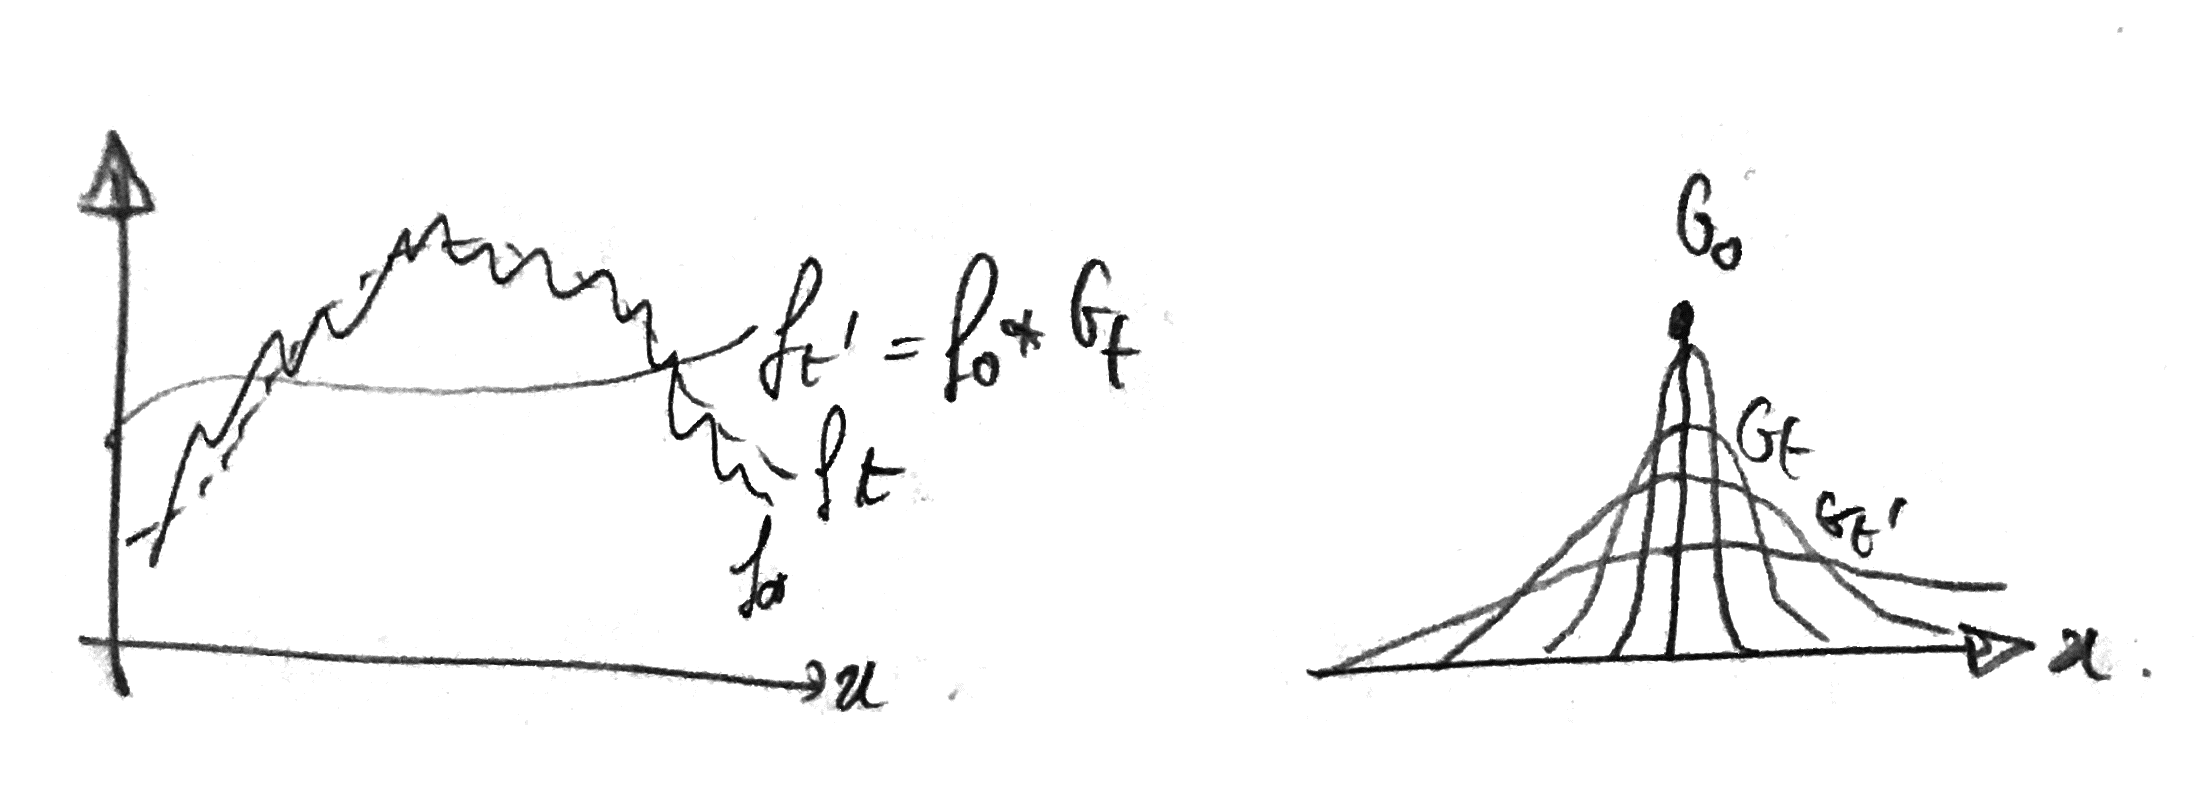
\includegraphics[width=.5\linewidth]{2-fourier/heat}
\caption{\label{fig-heat}
Heat diffusion as a convolution.
}
\end{figure}

As a typical example, we consider the heat equation
\eq{
	\frac{\partial f_t}{\partial t} = \Delta f_t
	\qarrq
	\foralls \om, \quad \frac{\partial \hat f_t(\om)}{\partial t} = -\norm{\om}^2 \hat f(\om).
}
This shows that $\hat f_t(\om) = \hat f_0(\om) e^{-\norm{\om}^2 t}$ and by inverse Fourier transform and the convolution theorem
\eq{
	f_t = G_t \star f_0 \qwhereq
	G_t=\frac{1}{(4\pi t)^{d/2}} e^{-\frac{\norm{x}^2}{4t}}
}
which is a Gaussian of standard deviation $\sqrt{2t}$.


%%%%%%%%%%%%%%%%%%%%%%%%%%%%%%%%%%%%%%%%%%%%%%%%
\subsection{Finite Domain and Discretization}

On $\RR/N\ZZ$ (i.e. discrete domains with periodic boundary conditions), one typically considers forward finite differences (first and second order)
\begin{align}\label{eq-disc-diff-1}
	D_1 f &\eqdef N (f_{n+1}-f_n)_n = f \star d_1 \qwhereq d_1 = [-1,0,\ldots,0,1]^\top \in \RR^N, \\
	\label{eq-disc-diff-2}
	D_2 f = D_1^\top D_1 f & \eqdef N^2 (f_{n+1}+f_{n-1}-2f_n)_n = f \star d_2 \qwhereq d_2 = d_1 \star \bar d_1 = [2,-1,0,\ldots,0,-1]^\top \in \RR^N.
\end{align}
\wrapf{2-fourier/finite-diff}{Comparison of the spectrum of $\De$ and $D_2$. }
Thanks to Proposition~\ref{prop-tfd-conv}, one can alternatively computes
\eq{
	\Ff( D_2 f ) = \hat d_2 \odot \hat f
	\qwhereq
	(\hat d_2)_k = N^2 ( e^{\piN} + e^{-\piN} - 2 ) = -4N^2 \sin\pa{\frac{\pi k}{N}}^2.
}
For $N \gg k$, one thus has $(\hat d_2)_k \sim -(2\pi k)^2$ which matches the scaling of~\eqref{eq-lapl-fourier}. 


%%%%%%%%%%%%%%%%%%%%%%%%%%%%%%%%%%%%%%%%%%%%%%%%
%%%%%%%%%%%%%%%%%%%%%%%%%%%%%%%%%%%%%%%%%%%%%%%%
%%%%%%%%%%%%%%%%%%%%%%%%%%%%%%%%%%%%%%%%%%%%%%%%
\section{A Bit of Group Theory}

The reference for this section is~\cite{peyre2004algebre}.

%%%%%%%%%%%%%%%%%%%%%%%%%%%%%%%%%%%%%%%%%%%%%%%%
\subsection{Characters}

For $(G,+)$ a commutative group, a character is a group morphism $\chi : (G,+) \rightarrow (\CC^*,\cdot)$, i.e. is satisfies
\eq{
	\foralls (n,m) \in G, \quad \chi(n+m) = \chi(n)\chi(m).
}
The set of characters is the so-called dual $(\hat G,\odot)$ and is a group for the pointwise multiplication $(\chi_1 \odot \chi_2)(n) \eqdef \chi_1(n) \chi_2(n)$.  Indeed, the inverse of a character $\chi$ is $\chi^{-1}(n)=\chi(-n)$.

Note that for a finite group $G$ with $|G|=N$, then since $N \times n=0$ for any $n \in G$, then $\chi(n)^N=\chi(N n)=\chi(0)=1$, so that characters assume values in the unit circle, and more precisely
\eql{\label{eq-char-finite-group}
	\chi(n) \in \enscond{ e^{\piN k} }{ 0 \leq k \leq N-1 }.
}
So in particular $\hat G$ is a finite group (since there is a finite number of application between two finite sets) and $\chi^{-1}=\bar\chi$. In the case of a cyclic group, the dual is actually simple to describe.

\begin{prop}\label{prop-iso-cyclic}
	For $G=\ZZ/N\ZZ$, then $\hat G=( \phi_k )_{k=0}^{N-1}$ where $\phi_k=( e^{\piN nk} )_n$ and $k \mapsto \phi_k$ defines a (non-canonical) isomorphism $G \sim \hat G$. 
\end{prop}
\begin{proof}
	The $\phi_k$ are indeed characters.
	
	Conversely, for any $\chi \in \hat G$, according to~\eqref{eq-char-finite-group}, $\chi(1)=e^{\piN k}$ for some $k$. Then 
	\eq{
		\chi(n)=\chi(1)^n=^{\piN k n} = \phi_k(n).
	}
	Note that all these applications are different (because $\phi_k(1)$ are all distincts) which shows that $|G|=|\hat G|$ so that they are isomorphic. 
\end{proof}

This proposition thus shows that characters of cyclic groups are exactly the discrete Fourier orthonormal basis defined in~\eqref{eq-dft}. 


%%%
\paragraph{Commutative groups.}

For more general commutative groups with a finite number of generators, according to the celebrated structure theorem, one can ``decompose'' them as a product of cyclic group (which are in some sense the basic building blocks), i.e. there is the following isomorphism of groups
\eql{\label{eq-structure}
	G \sim (\ZZ/N_1\ZZ) \times \ldots \times (\ZZ/N_d\ZZ) \times \ZZ^Q.
}
If $G$ is finite, then $Q=0$ and $N=N_1 \times N_d$. In this case, $G$ is simply a discrete $d$-dimensional ``rectangle'' with periodic boundary conditions. 

For two finite groups $(G_1,G_2)$ one has 
\eql{\label{eq-iso-product-char}
	\widehat{G_1 \times G_2} = \hat G_1 \otimes \hat G_2 = \enscond{ \chi_1 \otimes \chi_2 }{ (\chi_1,\chi_2) \in \hat G_1 \times \hat G_2 }.
} 
Here $\otimes$ is the tensor product of two functions
\eq{
	\foralls (n_1,n_2) \in G_1 \times G_2, \quad
	(\chi_1 \otimes \chi_2)(n_1,n_2) \eqdef \chi_1(n_1)\chi_2(n_2).
}
Indeed, one verifies that $\chi_1 \otimes \chi_2$ is a morphism, and in fact one has the factorization $\chi=\chi(\cdot,0) \otimes \chi(0,\cdot)$ because one decomposes $(n_1,n_2)=(n_1,0)+(0,n_2)$. 

This construction, thanks to the structure theorem, leads to a constructive proof of the isomorphism theorem.

\begin{prop}
	If $G$ is commutative and finite then $\hat G \sim G$.
\end{prop}
\begin{proof}
	The structure theorem~\eqref{eq-structure} for $Q=0$ and the dual of a product~\eqref{eq-iso-product-char} shows that 
	\eq{
		\hat G \sim \hat G_1 \otimes \ldots \otimes \hat G_d
	} 
	where we denoted $G_\ell \eqdef \ZZ/N_\ell\ZZ$. 
	%
	One then remark that  $\hat G_1 \otimes \hat G_2 \sim G_1 \times \hat G_2$.
	%
	One conclude thanks to Proposition~\ref{prop-iso-cyclic}, since one has $\hat G_k \sim G_k$.
\end{proof}

Note that the isomorphism $\hat G \sim G$ is not ``canonical'' since it depends on the indexing of the roots of unity on the circle. Similarly to the case of duality of vector space, the isomorphism $\hat{\hat{G}} \sim G$ can be made canonical by considering the evaluation map
\eq{
	g \in G \longmapsto e_g \in \hat{\hat{G}}
	\qwhereq
	\pa{
	e_g : \chi \in \hat G \mapsto \chi(g) \in \CC^*.
	}
}

%%%
\paragraph{Discrete Fourier transform from character's point of view.}

One can be even more constructive by remarking that characters in $\hat G_\ell$ are the discrete Fourier atoms~\eqref{eq-dft}, i.e. are of the form 
\eq{
	( e^{\frac{2\imath\pi}{N_\ell} k_\ell n_\ell})_{n_\ell=0}^{N_\ell-1}
	\quad\text{for some}\quad
	0 \leq k_\ell < N_\ell.
} 
Identifying $G$ and $G_1 \times \ldots \times G_d$, 
by tensorizing these functions together, one thus obtains that the characters composing $\hat G$ are exactly the orthogonal multi-dimensional discrete Fourier basis~\eqref{eq-exp-four-disc-multid}.

%%%%%%%%%%%%%%%%%%%%%%%%%%%%%%%%%%%%%%%%%%%%%%%%
\subsection{More General cases}

%%%
\paragraph{Infinite groups.}

For an infinite group with a finite number of generator, one has  $Q>0$, and the definition of $\hat G$ should impose the continuity of the characters (and also use an invariant measure on $G$ to define inner products). In the case $G=\ZZ$, the dual are indexed by a continuous parameter, 
\eq{
	\hat \ZZ = \enscond{ \phi_\om : n \mapsto e^{\imath n \om} \in L^2( \RR/2\pi\ZZ) }{  \om \in \RR/2\pi\ZZ }
}
so that $\hat \ZZ \sim \RR/2\pi\ZZ$.
%
The case $G=\ZZ^Q$ follows by tensorization. 
%
The $(\phi_\om)_\om$ are ``orthogonal'' in the sense that $\dotp{\phi_\om}{\phi_{\om'}}_\ZZ = \de(\om-\om')$ can be understood as a Dirac kernel (this is similar to the Poisson formula), where $\dotp{u}{v}_\ZZ \eqdef \sum_n u_n \bar v_n$. 
%
The ``decomposition'' of a sequence $(c_n)_{n \in \ZZ}$ on the set of characters is equivalent to forming a Fourier series $\sum_n c_n e^{-\imath n \om}$. 

Similarly, for $G=\RR/2\pi\ZZ$, one has $\hat G=\ZZ$, with orthonormal characters $\phi_n=e^{\imath \cdot n}$, so that the decomposition of functions in $L^2(G)$ is the computation of Fourier coefficients.

%%%
\paragraph{Non-commutative groups.}
 
For non-commutative group, one also observe that $G$ is not isometric to $\hat G$. A typical example is the symmetric group $\Si_N$ of $N$ elements, where one can show that $\hat G = \{\Id,\epsilon\}$ where $\epsilon(\si) = (-1)^{q}$ is the signature, where $q$ is the number of permutations involved in a decomposition of $\si \in \Si_N$. 

In order to study non-commutative groups, one has to replace morphisms $\chi : G \rightarrow \CC^*$ by morphisms $\rho : G \rightarrow \text{GL}(\CC^d)$ for some $d$, which are called ``representations'' of the group $G$. For $(g,g') \in G$ (denoting now multiplicatively the operation on $G$), one should thus have $\rho(gg')=\rho(g) \circ \rho(g')$. When $d=1$, identifying $\text{GL}(\CC) \sim \CC^*$, one retrieve the definition of characters. Note that if $\rho$ is a representation, then $\chi(g) \eqdef \tr(\rho(g))$, where $\tr$ is the trace, defines a character. 
%
In order to limit the set of such representations, one is only interested in ``elementary'' ones, which does not have invariant sub-spaces, and are called ``irreducible'' (otherwise one could create arbitrary large representation by stacking others in a block diagonal way). 
%
One can show that the dimensions of these irreducible representations sum to $N$ and that the entries of the matrices involved in these representation define an orthogonal basis of the space of functions $f : G \rightarrow \CC$, thus leading to a theory extending the one on commutative groups. In particular, this Fourier transform in some sense also diagonalizes convolutions over $G$
\eq{
	f \star h(a) \eqdef \sum_{bc=a} f(b) h(c).
}
%
For the symmetric group, there is an explicit description of the set of irreducible representations.  
 
 

%%%%%%%%%%%%%%%%%%%%%%%%%%%%%%%%%%%%%%%%%%%%%%%%
%%%%%%%%%%%%%%%%%%%%%%%%%%%%%%%%%%%%%%%%%%%%%%%%
%%%%%%%%%%%%%%%%%%%%%%%%%%%%%%%%%%%%%%%%%%%%%%%%
\section{A Bit of Spectral Theory}

In order to define Fourier methods on general domains $\XX$, one can use the aforementioned group-theoretic approach if $\XX=G$ is a group, or also if a group acts transitively on $\XX$. An alternative way is to describe the equivalent of Fourier basis functions as diagonalizing a specific differential operator (as we have seen in Section~\ref{sec-fourier-pdes}�that it is in some sense a way to characterise the Fourier basis). Of particular interest is the Laplacian, since it is the lowest order rotation-invariant differential operator, and that there exists natural generalization on domains such as surfaces or graphs.


%%%%%%%%%%%%%%%%%%%%%%%%%%%%%%%%%%%%%%%%%%%%%%%%
\subsection{On a Surface or a Manifold}

\wrapf{2-fourier/laplacian-surf}{Computing Laplacian on a surface}
The presentation here is very informal. One can define the Laplacian of a smooth function $f: \XX \rightarrow \CC$ defined on a ``surface'' $\XX$ as
\eq{
	\foralls x \in \XX, \quad
	(\Delta f)(x) \eqdef \lim_{\epsilon \rightarrow 0}  \frac{1}{\text{Vol}(B_\epsilon(x))} \int_{B_\epsilon(x)} f(x) \d \mu(x) - f(x).
}
Here $\mu(x)$ is the area measure on $\XX$, $\text{Vol}(B) \eqdef \int_B \d\mu(x)$, and $B_\epsilon(x) = \enscond{y}{d_\XX(x,y) \leq \epsilon}$ is the geodesic ball of radius $\epsilon$ at $x$, where $d_\XX$ is the geodesic distance on $\XX$ (length of the shortest path). 

If the surface $\XX$ is smooth, compact and connected, then it is possible to show that $\Delta$ is itself a compact operator with a negative spectrum $0 > \la_1 > \la_2 > \ldots$ and an orthogonal set of eigenvectors $(\phi_n)_{n \geq 0}$ where $\phi_1=1$. Here the inner product is $\dotp{f}{g}_\XX \eqdef \int_\XX f(x)g(x) \d\mu(x)$ on $L^2(\XX)$. 
%
In the case of a flat torus $\XX=(\RR/\ZZ)^d$, then writing $x=(x_1,\ldots,x_d)$, 
\eq{
	\De f = \sum_{s=1}^d \frac{\partial^2 f}{\partial^2 x_s}.
} 
Similarly to~\eqref{eq-lapl-fourier} (which was for an unbounded domain), then one can chose for this eigen-functions $\phi_n$ the Fourier basis~\eqref{eq-fourier-basis-1d} and $\la_n=-\norm{n}^2$

%%%%%%%%%%%%%%%%%%%%%%%%%%%%%%%%%%%%%%%%%%%%%%%%
\subsection{Spherical Harmonics}

\wrapf{2-fourier/spherical}{Spherical coordinates.}
Of particular interest is the special case of the previous construction on the $(d-1)$-dimensional sphere $\SS^{d-1} = \enscond{x \in \RR^d}{\norm{x}_{\RR^d}=1}$.
% 
In this case, there exists a closed form expression for the eigenvectors of the Laplacian. In the 3-D case $d=3$, they are indexed by $n=(\ell,m)$
\eq{
	\foralls \ell \in \NN, \quad
	\foralls m=-\ell,\ldots,\ell, \quad
	\phi_{\ell,m}(\th,\phi) = e^{\imath m \phi} P_{\ell}^m( \cos(\th) )
}
and then the eigenvalue of the Laplacian is $\la_{\ell,m} = -\ell(\ell+1)$. Here $P_{\ell}^m$ are associated Legendre polynomials, and we used spherical coordinates $x=(\cos(\phi),\sin(\phi)\sin(\th),\sin(\phi)\cos(\th)) \in \SS^3$ for $(\th,\phi) \in [0,\pi] \times [0,2\pi]$.
%
The index $\ell$ is analogous to the amplitude of Fourier frequencies in 2-D. 
%
For a fixed $\ell$, the space $V_\ell = \text{span}( \phi_{\ell,m} )$ is an eigenspace of $\Delta$, and is also invariant under rotation. 
	

%%%%%%%%%%%%%%%%%%%%%%%%%%%%%%%%%%%%%%%%%%%%%%%%
\subsection{On a Graph}

\wrapf{2-fourier/graph}{Weighted graph.}
We assume $\XX$ is a graph of $N$ vertices, simply indexed $\{1,\ldots,N\}$. Its ``geometry'' is described by a connectivity matrix of weights $W=(w_{i,j})_{i \sim j}$ where we denote $i \sim j$ to indicate that $(i,j)$ is an edge of the graph for $(i,j) \in \XX^2$. We assume that this weight matrix and the connectity is symmetric, $w_{i,j}=w_{j,i}$. 

The graph Laplacian $\Delta : \RR^N \rightarrow \RR^N$ is computing the difference between the average of values around a point and the value at this point
\eq{
	\foralls f \in \RR^N, \quad
	(\Delta f)_i \eqdef \sum_{j \sim i} w_{i,j} f_j - (\sum_{j \sim i} w_{i,j}) f_i 
	\qarrq 
	\Delta = W-D
}
where $D \eqdef \diag_i(\sum_{j \sim i} w_{i,j})$. In particular, note $\Delta \ones=0$

For instance, if $\XX = \ZZ/N\ZZ$ with the graph $i \sim i-1$ and $i \sim i+1$ (modulo $N$), then $\De$ is the finite difference Laplacian operator $\De=D_2$ defined in~\eqref{eq-disc-diff-2}. This extends to any dimension by tensorization. 

\begin{prop}
Denoting $G : f \in \RR^N \mapsto ( \sqrt{w_{i,j}} (f_i-f_j) )_{i<j}$ the graph-gradient operator, one verifies that 
\eq{
	-\Delta = G^\top G
	\qarrq
	\foralls f \in \RR^N, \quad 
	\dotp{ \Delta f }{f}_{\RR^N} = -\dotp{Gf}{Gf}_{\RR^{P}}.
}
where $P$ is the number of (ordered) edges $E=\enscond{(i,j)}{i \sim j, i<j}$. 
\end{prop}
\begin{proof}
	One has 
	\begin{align*}
		\norm{Gf}^2 &= \sum_{(i,j) \in E} w_{i,j}|f_i-f_j|^2
				=\sum_{i<j}w_{i,j}f_i^2  + \sum_{i<j}w_{i,j}f_j^2 - 2 \sum_{i<j}w_{i,j}f_i f_j  \\
				&= \sum_{i<j}w_{i,j}f_i^2 + \sum_{i>j}w_{i,j}f_i^2- \sum_{i,j}w_{i,j}f_i f_j
				= \sum_j f_i^2 \sum_{i,j} w_{i,j} - \sum_if_i  \sum_j w_{i,j} f_j \\
				&= \dotp{Df}{f}-\dotp{Lf}{f}=-\dotp{Lf}{f}.
	\end{align*}
\end{proof}

This proposition shows that $\Delta$ is a negative semi-definite operator, which thus diagonalizes in an ortho-basis $(\phi_n)_{n=1}^N$, with $\phi_1=1$, with eigenvalues $0 \geq \la_1 \geq \la_N$. If $\XX$ is connected, one can show that $\la_1 <0$. In the case of a regular graph associated to a uniform grid, one retrieves the discrete Fourier basis~\eqref{eq-dft}. 

More details and application of Laplacians on graphs can be found in Chapter~\ref{chap-meshes}, see in particular Section~\ref{sec-grad-lapl-meshes}.




